\documentclass[notitlepage]{report}

\usepackage{graphicx}
\usepackage{titling}
\usepackage{pgfplotstable}
\pgfplotsset{compat=1.15}
\usepackage{longtable}

\setlength{\droptitle}{-10em}

\title{CUDA Monte Carlo}
\author{Sudha Ravi Kumar Javvadi}

\begin{document}
	\maketitle
	
	\paragraph{Introduction}
	\paragraph{} Monte Carlo simulation is used to determine the range of outcomes for a series of parameters. In this project Monte Carlo simulation is implemented to determine the probability of a beam hitting a circular plate when it is randomly changing location and size. The report documents this attempt when run on CUDA.
	
	\paragraph{Machine Details}
	\begin{itemize}
		\item{OS}: Ubuntu 18.04.04 LTS
		\item{Memory}: 15.5 GB
		\item{Processor}: Intel Core i5-9600K CPU @ 3.70GHz x 6
		\item{Graphics}: GeForce RTX 2070 SUPER/PCIe/SSE2
		\item{GNOME}: 3.28.2
		\item{OS type}: 64-bit
		\item{Disk}: 225.4 GB
		\item{CUDA}: 10.2
	\end{itemize}

	\paragraph{Results}
	\paragraph{}
	\pgfplotstableset{
		begin table=\begin{longtable},
			end table=\end{longtable},
	}
	\pgfplotstabletypeset[
		col sep=comma,
		string type,
		columns/trials/.style={column name=Trials, column type={|c}},
		columns/size/.style={column name=Size, column type={c|}},
		columns/performance/.style={column name=Performance, column type={c}},
		columns/probability/.style={column name=Probability, column type={c|}},
		every head row/.style={before row={
				\caption{Table showing speedups with SIMD over non-SIMD}
				\label{tab:sim}\\
				\hline},
			after row=\hline},
		every last row/.style={after row=\hline},
	]{../data/simulations.csv}
	An attempt to explain the simulation result in table \ref{tab:sim} is done with the help of following graphs in figures \ref{fig:size} and \ref{fig:trials}. Please note that the performance is calculated as mega trials simulated per second.
	
	\paragraph{Performance vs Block Size}
	\paragraph{}
	\begin{figure}[!ht]
		\includegraphics [width=\linewidth] {../data/trials.png}
		\caption{Performance of CUDA Monte Carlo}
		\label{fig:trials}
	\end{figure}
	\paragraph{} Figure \ref{fig:trials} plots Performance vs Block Sizes for a number of trials. It can be observed that there is better performance with increasing number of trials. As the number of trials increase there is more data to deal with and so the improved performance because GPUs are meant to work better with specific size range of large data. It can also be noted that the performance increases initially when the block size is increased to 32, but then it is either almost the same or drops down a little as the block size is increased through 128. This might be because of increased thrashing of data in and out of memory.
	
	\paragraph{Performance vs \# of Trials}
	\paragraph{}
	\begin{figure}[!ht]
		\includegraphics [width=\linewidth] {../data/size.png}
		\caption{Performance of CUDA Monte Carlo}
		\label{fig:size}
	\end{figure}
	\paragraph{} Figure \ref{fig:size} plots Performance vs Number of Trials for different block sizes. It can be observed that the performance is almost similar for different block sizes except when the block size is 16. The performance is worst when block size is 16. Total number of threads in a warp is 32, where all 32 threads execute a single instruction at the same time. Setting the block size to 16 is forcing the GPU to execute less number of similar instructions at a time in a warp. In other words it has less occupancy. Whereas setting the block size to more than or equal to 32 but a multiple of 32 can be spread across multiple warps with good occupancy. This could be the possible reason for the worst performance with block size equals 16.
	
	\paragraph{Comparison with Project \#1 results}
	\paragraph{}
	\begin{figure}[!ht]
		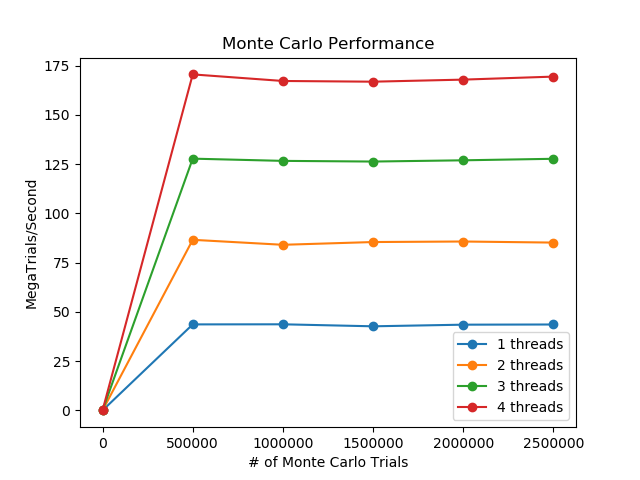
\includegraphics [width=\linewidth] {proj1.png}
		\caption{Performance of Monte Carlo}
		\label{fig:cpu}
	\end{figure}
	\paragraph{} Figure \ref{fig:cpu} plots Performance vs Number of Trials for different number of threads when run on a CPU. Please note that the above graph is taken from my project 1 submitted report. Comparing figures \ref{fig:size} and \ref{fig:cpu}, it can be observed that the number of mega trials simulated per second is almost 17 times on GPU than on CPU. I think even if the number of threads were increased by 4 times, the performance of CPU cannot beat that of a GPU. This proves that the GPUs can parallelise execution of similar instructions but on different data. So, the computations on large datasets is faster on GPUs than on CPUs.
	
	\paragraph{Code}
	\paragraph{} Please unzip the file and run $./start.sh$ in the project folder to see the results and also populate the report.
	\paragraph{} Also, all the other details on structure of the code can be found in \textit{README.md} in the project folder.
\end{document}
